% !TeX root = main.tex
\changecolours{ScoutPurple}
\section[Aggregation e Desafio Integrado]{Aggregation Framework, Performance e Desafio Prático}

% ------------------------------------------------------------------------------
\begin{frame}[fragile]{Revisão do Aggregation Framework: Estrutura em Pipeline}
  \vspace{0.1cm}
  \begin{columns}[t,onlytextwidth]
    \begin{column}{0.48\textwidth}
      \alert{Estágios Críticos do Pipeline}\par
      \footnotesize
      \begin{itemize}
        \item \lstinline[language=mongosh, basicstyle=\footnotesize\ttfamily]|$match|: redução inicial volumétrica via índice $B\text{-Tree}$.
        \item \lstinline[language=mongosh, basicstyle=\footnotesize\ttfamily]|$unwind|: desconstrução de arrays para permitir agregações por item.
        \item \lstinline[language=mongosh, basicstyle=\footnotesize\ttfamily]|$group|: agrupamento por chave e acumuladores (\lstinline[language=mongosh, basicstyle=\footnotesize\ttfamily]|$sum|, \lstinline[language=mongosh, basicstyle=\footnotesize\ttfamily]|$avg|).
        \item \lstinline[language=mongosh, basicstyle=\footnotesize\ttfamily]|$sort| e \lstinline[language=mongosh, basicstyle=\footnotesize\ttfamily]|$limit|: ordenação determinística e paginação.
      \end{itemize}
    \end{column}
    
    \begin{column}{0.50\textwidth}
      \alert{Pipeline Analítico no MongoSH}\par
      \vspace{0.05cm}
      \begin{lstlisting}[language=mongosh]
// Relatorio de faturamento por categoria
db.pedidos.aggregate([
  { $match: { status: "ENTREGUE" } },
  { $unwind: "$itens" },
  {
    $group: {
      _id: "$itens.categoria",
      receita: { $sum: "$itens.subtotal" },
      unidades: { $sum: "$itens.quantidade" }
    }
  },
  { $sort: { receita: -1 } }
]);
      \end{lstlisting}
    \end{column}
  \end{columns}
\end{frame}

% ------------------------------------------------------------------------------
\begin{frame}{Evidência Empírica: Latência Poliglota Integrada}
  \vspace{0.1cm}
  \begin{columns}[t,onlytextwidth]
    \begin{column}{0.48\textwidth}
      \alert{Comparativo das Camadas de Acesso}\par
      \footnotesize
      \begin{itemize}
        \item \textbf{Redis (RAM):} $\approx 0.08\text{ ms}$ (acesso $\mathcal{O}(1)$ via chave direta). Mais de $200\times$ mais rápido que disco.
        \item \textbf{MongoDB Indexado ($B\text{-Tree}$):} $\approx 1.15\text{ ms}$ ($\mathcal{O}(\log N)$ via índice composto ESR).
        \item \textbf{MongoDB sem Índice (\texttt{COLLSCAN}):} $\approx 18.4\text{ ms}$ ($\mathcal{O}(N)$ varredura linear de $10.000$ docs).
      \end{itemize}
      
      \vspace{0.15cm}
      \alert{Conclusão de Arquitetura}\par
      A arquitetura de cache-aside combina a velocidade em RAM do Redis com a persistência de documentos do MongoDB.
    \end{column}
    
    \begin{column}{0.50\textwidth}
      \alert{Medição Empírica (Tempo de Resposta)}\par
      \vspace{0.05cm}
      \centering
      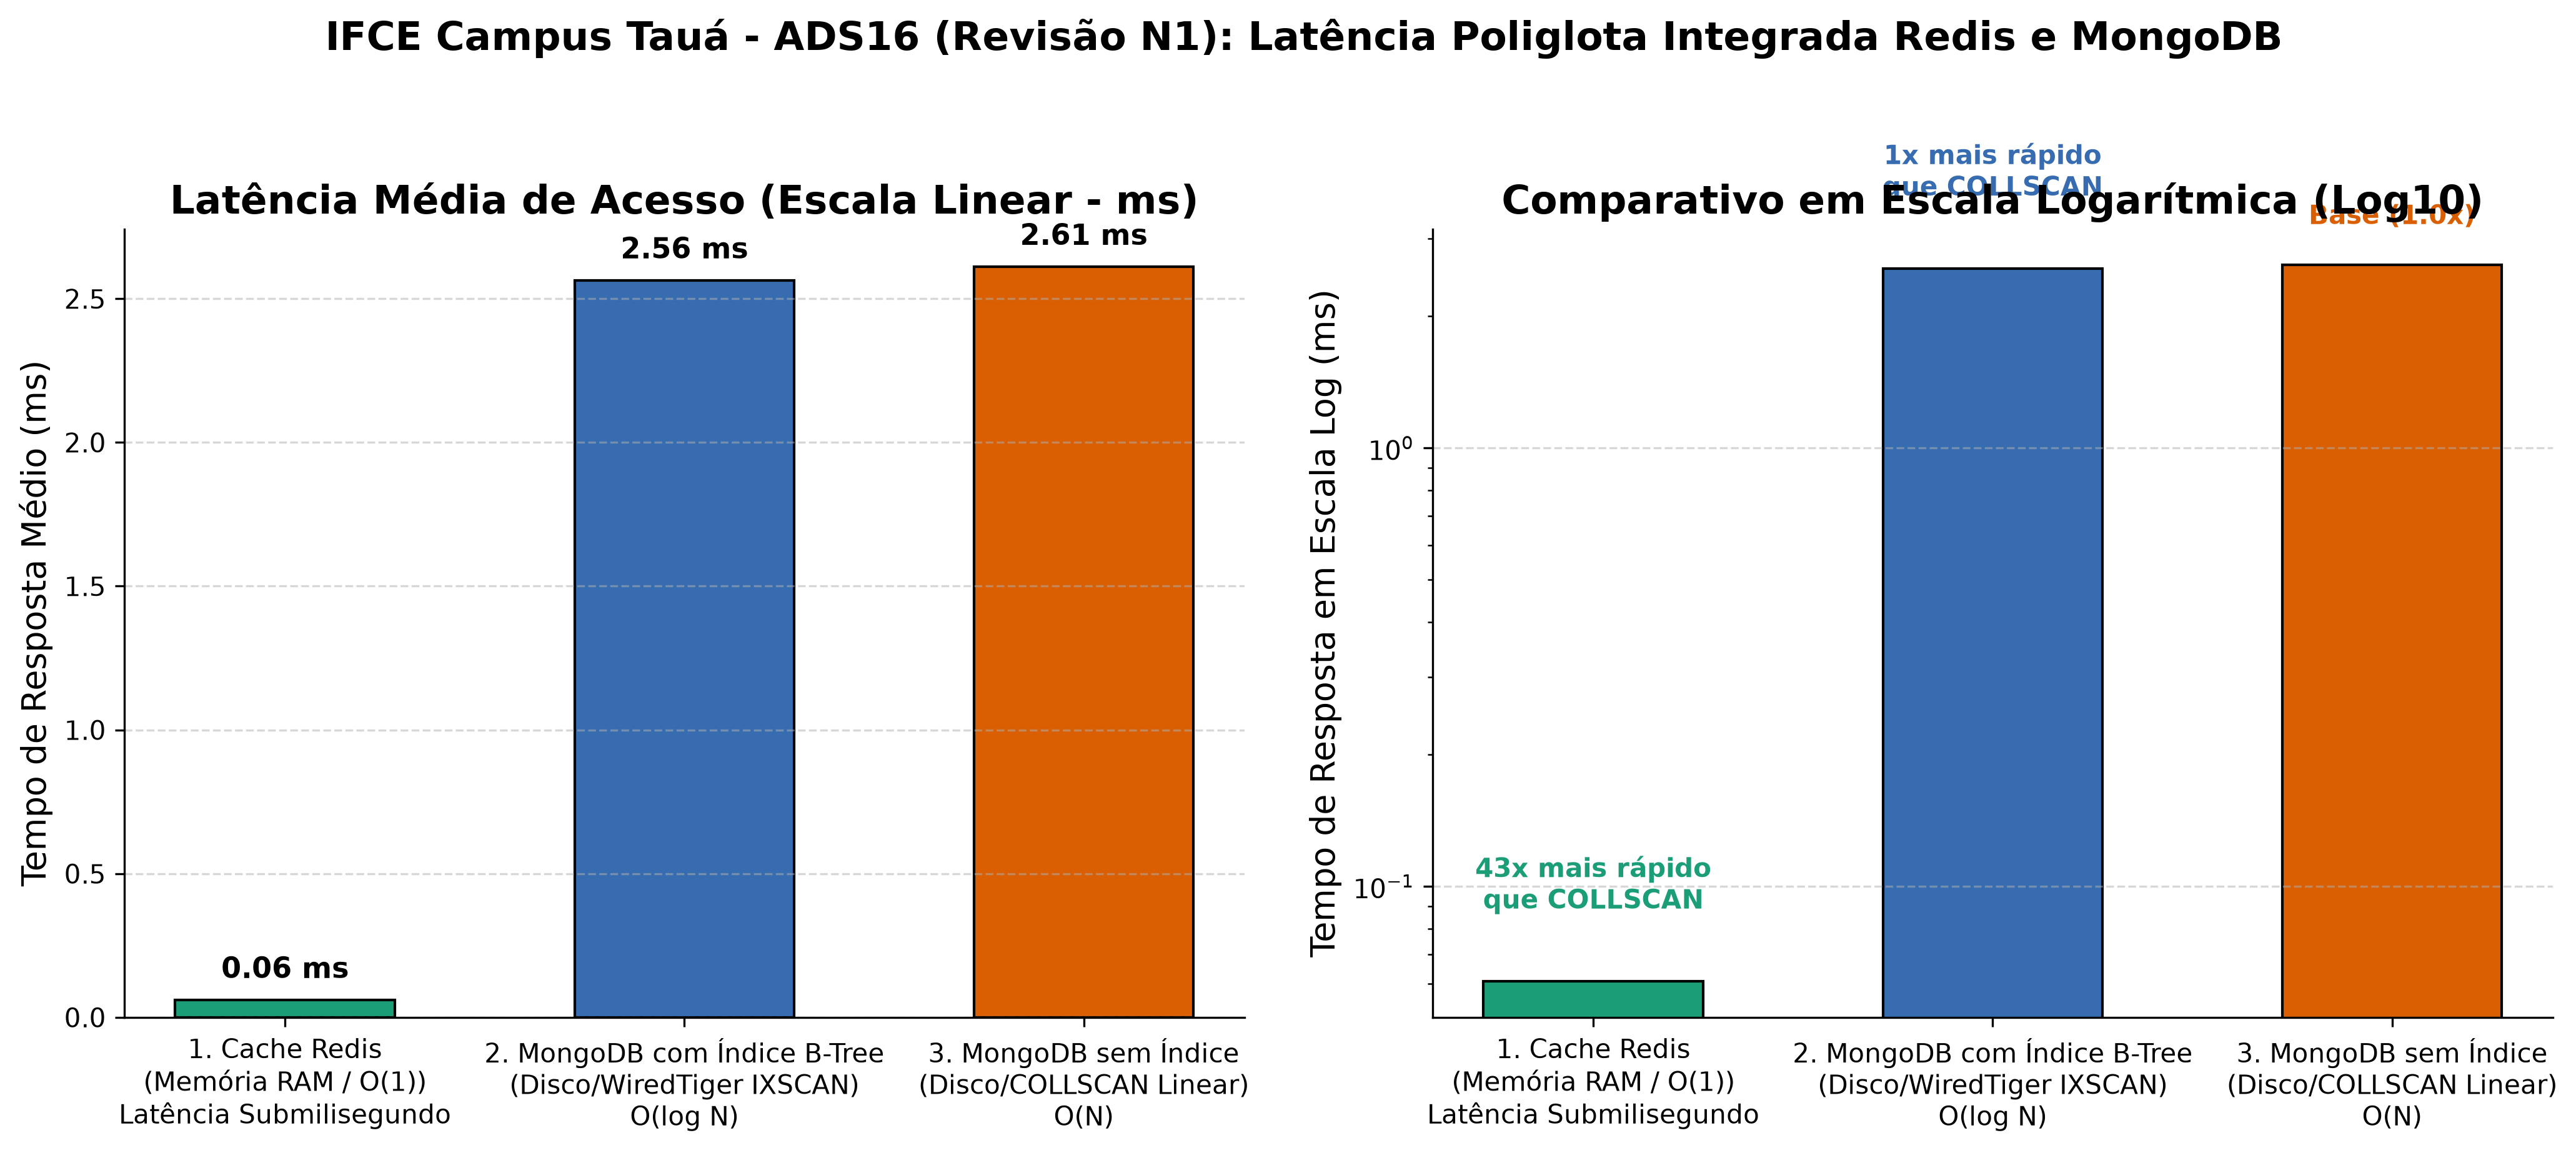
\includegraphics[width=\linewidth, height=4.2cm, keepaspectratio]{benchmark_latencia_revisao.png}
    \end{column}
  \end{columns}
\end{frame}

% ------------------------------------------------------------------------------
\begin{frame}[fragile]{Diretrizes para o Simulado Prático (AVP1)}
  \vspace{0.1cm}
  \begin{columns}[t,onlytextwidth]
    \begin{column}{0.48\textwidth}
      \alert{Como Realizar o Simulado em Laboratório}\par
      \footnotesize
      \begin{enumerate}
        \item Inicie os serviços locais via Docker Compose:
          \par\vspace{0.08cm}
          \centering
          \lstinline[language=mongosh, basicstyle=\scriptsize\ttfamily]|docker compose up -d|
          \par\vspace{0.08cm}
          \raggedright
        \item Abra o script \texttt{simulado\_n1\_desafios.py}.
        \item Resolva os 5 desafios sequencialmente.
        \item Valide suas respostas executando o script:
          \par\vspace{0.08cm}
          \centering
          \lstinline[language=mongosh, basicstyle=\scriptsize\ttfamily]|python3 simulado_n1_desafios.py|
          \par\vspace{0.08cm}
          \raggedright
      \end{enumerate}
    \end{column}
    
    \begin{column}{0.48\textwidth}
      \alert{Critérios de Avaliação da AVP1 (Aula 10)}\par
      \footnotesize
      \begin{itemize}
        \item \textbf{Integração Poliglota:} Lógica de leitura/escrita coordenada entre Redis e MongoDB.
        \item \textbf{Cache-Aside com TTL:} Consulta primária ao cache e hidratação com expiração temporal.
        \item \textbf{Operadores Atômicos:} Modificação de concorrência com \lstinline[language=mongosh, basicstyle=\footnotesize\ttfamily]|$inc| e \lstinline[language=rediscli, basicstyle=\footnotesize\ttfamily]|HINCRBY|.
        \item \textbf{Indexação ESR:} Justificativa técnica da ordem dos campos no índice composto.
      \end{itemize}
    \end{column}
  \end{columns}
\end{frame}
